% To begin the document, load the 'knac' document class, which is a
% modified version of the AASTeX class.  Documentation for that
% package is available at http://aas.org/aastex/aastex-documentation.
%
% In your document, you can use almost any of the new LaTeX commands
% defined by the AASTeX package (e.g. \deluxetable, \ion, \lesssim,
% \sun, \arcmin, \micron, \citep, \bibitem, \apj, etc.  The main
% exceptions are AASTeX commands that are specific to publishing a
% journal article, e.g.  \received, \revised, \accepted, \slugcomment,
% \keywords, etc.  But almost any text-markup command should be OK.

\documentclass{knac}

\usepackage{gensymb}
%  If you want to define shortcuts for commonly-typed commands you'll
%  use, you can do so here - for example, here is a command to make it
%  easier to refer to H alpha emission (using 'math mode', denoted by
%  the dollar signs, to generate the Greek letter alpha).

\begin{document}

\title{Simulating Observations Within the TRAPPIST-1 System}


\author{Girish Duvvuri, ASTR5810 Final Project}

\begin{abstract}
    Three of the seven known planets in the TRAPPIST-1 exoplanetary system lie in the Goldilocks zone for liquid surface water. Here we use model emission spectra from \cite{Morley2017} to simulate what one of these planets may be able to observe of another over a range of spectrograph resolutions, telescope collecting areas, exposure times, throughput efficiencies, and observing qualities parameterized by uncorrelated noise.
\end{abstract}

\section{Introduction}

The TRAPPIST-1 system consists of at least seven small roughly Earth-sized planets orbiting an ultracool M-dwarf star. Of these seven, three lie within the star's roughly defined Goldilocks zone for liquid surface water. These planets are prime candidates for further study with transmission spectroscopy with \emph{JWST}, and so \cite{Morley2017} presented model emission spectra for planets in this system for a variety of assumed surface pressures, compositions, and albedos. When the system's discovery was announced, I wondered what it would be like if sapient civilizations emerged on two neighbor planets. How would they see each other and at what point might one definitively recognize the other as alien life? This project answers a much simpler version of those questions: given the emission spectra of TRAPPIST-1 f and g, how would TRAPPIST-1 f observe TRAPPIST-1 g?

\section{Emission Spectra}
For TRAPPIST-1 f (the observer planet, where ``we" are standing), I use the model that assumes an Earth-like atmospheric composition, has a bond albedo $A_B = 0.3$, and surface pressure $P_\mathrm{surf} = 1$ bar. For TRAPPIST-1 g (our target planet), I selected the model with a Titan-like atmospheric composition, $A_B = 0$, and $P_\mathrm{surf} = 0.001$ bar. Since the albedo is set to 0, we can neglect any reflectance from the host star and do not need to consider TRAPPIST-1's spectrum for this simulation.

The emission spectrum models show the flux emitted from the top of the atmosphere of their respective planet both of which are shown in Figure \ref{figure:emission_spectra}. An algebraic expression for this flux is given by
\begin{equation}
F_\lambda = \left(B_{\lambda}(T_\mathrm{surf})e^{-\tau_\lambda} + \int_{0}^{\tau_\lambda} B_\lambda (T_{\tau_{\lambda}'})e^{-\tau_{\lambda}'}d\tau_{\lambda}' \right)\times 2\pi\left(1 - \cos{\theta}\right)
\label{equation:f_lambda}
\end{equation} where $\tau_\lambda$ is the optical depth through the whole atmosphere, $T_\mathrm{surf}$ is the surface temperature of the planet, $\theta$ is the angular radius of the planet, and $T(\tau_{\lambda}')$ is the temperature of a thin slab of atmosphere with optical depth $\tau_{\lambda}'$.


\begin{figure}[bht]
\centering
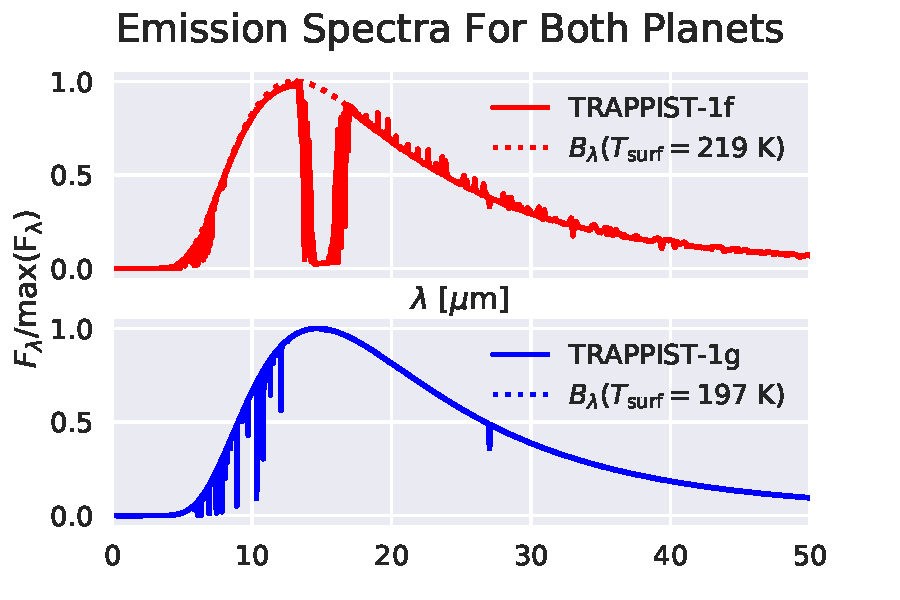
\includegraphics[angle=0,scale=0.82]{emission_both.pdf}
\caption{The model spectrum for the observer planet, TRAPPIST-1 f, is shown in the top subplot with the solid red line. The model spectrum for the target planet, TRAPPIST-1 g, is shown in the bottom subplot with the solid blue line. For both, we fit a blackbody radiation curve to find the surface temperature and plot the corresponding fit with a dotted line of the same color as the spectrum.}
\label{figure:emission_spectra}
\end{figure}

\section{Observing Atmosphere Contribution}
None of this matters for the target planet since we know the flux we receive is simply the given model emission spectra. But to account for the atmosphere we are looking through, we must know what flux our own atmosphere on TRAPPIST-1 f emits down towards our telescope pointed at TRAPPIST-1 g. Assuming an isotropically emitting atmosphere that does not scatter the radiation emitted by the ground back down to us, along with the more realistic assumption that we are observing at night and the sky is not scattering TRAPPIST-1's starlight, this atmospheric emission is given by the integral term in Equation \ref{equation:f_lambda}. Unfortunately, \cite{Morley2017} does not provide the temperature-pressure profile or $\tau_\lambda$ for each model, only the final emission spectrum product.

Conveniently, there is a very strong absorption feature at $\sim15 \mu$m that we can safely assume shows the greatest optical depth along the entire spectrum. If we label the optical depth at this absorption feature $\tau_{\lambda_{\mathrm{max}}}$ and assume the temperature follows a simple linear trend from $T_{\mathrm{skin}}$ at the top of the atmosphere to $T_{\mathrm{surf}}$ at the surface, tracking the optical depth from $0$ to $\tau_{\lambda_{\mathrm{max}}}$, we can express $T(\tau_{\lambda}')$ as
\begin{equation}
\label{equation:temp}
T(\tau_{\lambda}') = T_{\mathrm{skin}} + \frac{T_{\mathrm{surf}} - T_{\mathrm{skin}}}{\tau_{\lambda_{\mathrm{max}}}}\times \tau_{\lambda}'.
\end{equation}

Then we use a Taylor expansion to make the integral term analytical and use the model spectrum to give us $F_\lambda$, turning Equation \ref{equation:f_lambda} into a transcendental equation we can solve for $\tau_\lambda$. Given $\tau_\lambda$ (shown in Figure \ref{figure:tau}) and our linear temperature profile (Equation \ref{equation:temp}), we can solve for the integral term
\begin{equation}
    \text{Observer Atmosphere Specific Intensity} = \int_{0}^{\tau_\lambda} B_\lambda (T_{\tau_{\lambda}'})e^{-\tau_{\lambda}'}d\tau_{\lambda}'.
    \label{equation:background_integral}
\end{equation}

\begin{figure}[bht]
\centering
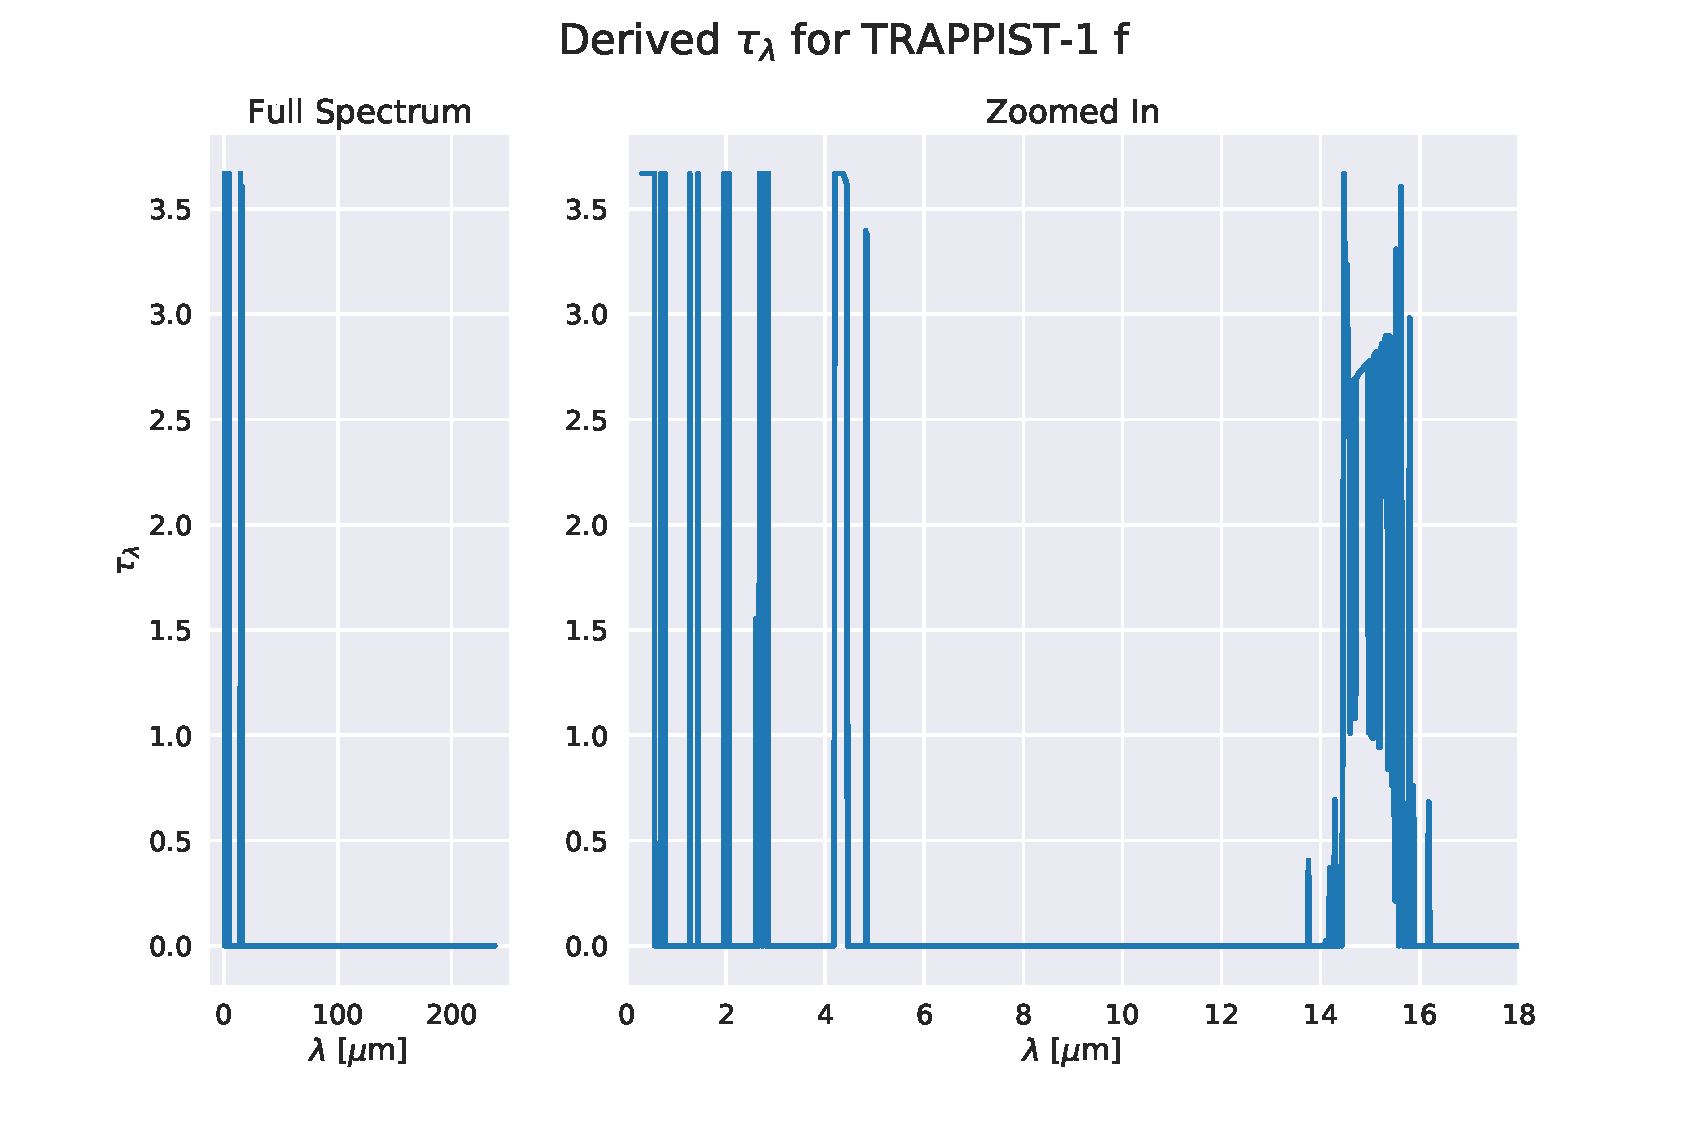
\includegraphics[angle=0,scale=0.4]{tau_lambda.pdf}
\caption{The left panel shows the optical depth over the whole spectrum while the right zooms into the absorption feature $\sim 15 \mu$m. The fact that the optical depth does not go to $\tau_{\lambda_{\mathrm{max}}}$ in the middle of the feature shows that this is a rough approximation at best.}
\label{figure:tau}
\end{figure}

\section{Signal-to-Noise Ratio Derivation}
The model provided must be consistent with the spectrograph we observe with, so we convolve it with a Gaussian kernel to match the resolution we assume, and then multiply by the throughput of the telescope ($f$, letting through anywhere between 0\% and 100\% of the light). The flux we observe from our target is this convolved emission spectrum of TRAPPIST-1 g modified by the angular size of the target, the collecting area of our telescope ($A$), and the exposure time ($t$):
\begin{equation}
\mathrm{Signal} = \left(F_\lambda * G(\frac{\lambda_\mathrm{mean}}{R})\right) \times \frac{\pi R_p^2}{4\pi d^2} \times A \times t \times f \times\frac{\lambda}{hc}
\end{equation} where $R_p$ is the radius of TRAPPIST-1 g and $d$ is the distance between TRAPPIST-1 f and g, which we assume is simply the difference between their orbital distances (TRAPPIST-1 g is at perfect opposition to us and both planets are on perfectly circular orbits).

The noise is a combination of the Poisson noise of our signal, the Poisson noise of the flux from our own atmosphere which we circuitously (and only approximately) solved for above, and white noise due to instrumental limitations ($\sigma^2$):
\begin{equation}
 \mathrm{Noise} = \sqrt{\mathrm{Signal} + \left(\int_{0}^{\tau_{\lambda}} B_{\lambda} (T_{\tau_{\lambda}'})e^{-\tau_{\lambda}'}d\tau_{\lambda}' \times f \times A \times t\times 2\pi\left(1 - \cos{\theta}\right)\right)\times\frac{\lambda}{hc} + \sigma^2}
\end{equation}

Then the SNR is simply:
\begin{equation}
    \mathrm{SNR} = \frac{\mathrm{Signal}}{\mathrm{Noise}}
\end{equation}

For the purposes of our simulation, the parameters we can vary are $R, f, t, A, \text{ and }\sigma^2$. Of these, $A$ we vary by changing the diameter of the telescope, and use $\log{\sigma^2}$ and $\log{R}$ instead of the values directly. For a wavelength range between $\lambda_\mathrm{min}$ and $\lambda_\mathrm{max}$ we can show the SNR as a function of wavelength and the true SNR is a mean over this function. In the project notebook, we allow these parameters to be varied and show the mean SNR integrated over the range specified using an interactive widget. A few example outputs from (an old version of) the widget are shown in Figure \ref{figure:widget_all} along with an explanation of the slider parameters in Figure \ref{figure:widget_slider}.
Looking at outputs from the most recent version of the widget
(moving from flux units to photons correctly), a very simple spectrograph
with high $\sigma^2 \sim 10^{35}$ photons can still detect absorption
features with high SNR.
\begin{figure}
    \centering
        \begin{minipage}{.33\textwidth}
        \centering
        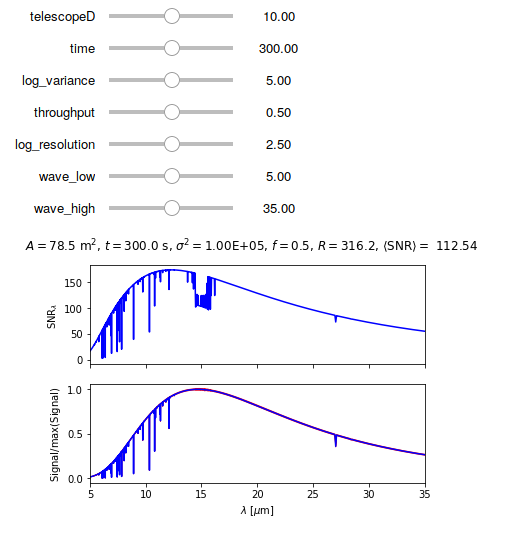
\includegraphics[width=1.0\linewidth]{widget_1.png}
    \end{minipage}%
    \begin{minipage}{0.33\textwidth}
        \centering
        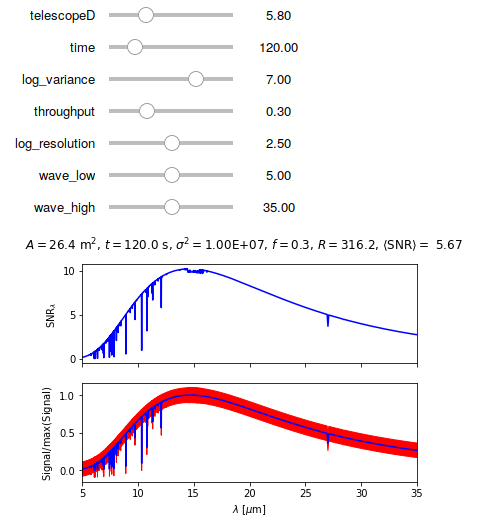
\includegraphics[width=1.0\linewidth]{widget_2.png}
    \end{minipage}
    \begin{minipage}{0.33\textwidth}
        \centering
        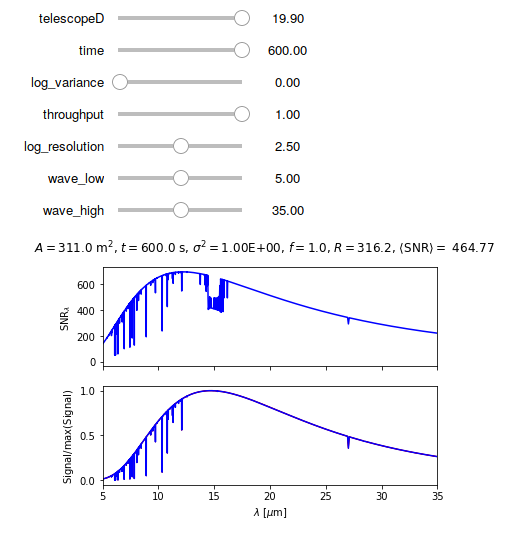
\includegraphics[width=1.0\linewidth]{widget_3.png}
    \end{minipage}
    \caption{For each figure, the top subplot shows SNR at each $\lambda$,
    and the bottom shows the signal received in blue with a red band indicating
    the range of noise (normalized by the maximum signal).
    The notebook has an updated form of this figure where a third plot is
    added below to represent the expected flux with injected noise
    corresponding to the calculated SNR (this noise is injected as a Gaussian
    with the variance determined by the SNR which is not strictly
    mathematically valid).}
    \label{figure:widget_all}
\end{figure}

\begin{figure}[h!]
\centering
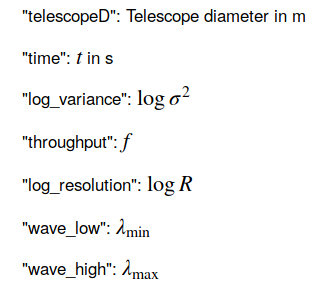
\includegraphics[scale=0.6]{widget_slider.png}
\caption{This figure expands the names of the slider parameters above the plots in Figure \ref{figure:widget_all}.}
\label{figure:widget_slider}
\end{figure}


\begin{thebibliography}{}

\bibitem[Morley et al.(2017)]{Morley2017} Morley, C.~V., Kreidberg, L., Rustamkulov, Z., Robinson, T., \& Fortney, J.~J.\ 2017, \apj, 850, 121

\end{thebibliography}

\end{document}
